\documentclass{article} % Changed from standalone to article for a full document
\usepackage[utf8]{inputenc}
\usepackage{pgfplots}
\pgfplotsset{compat=1.18}
\usepackage{amsmath,stackengine}
\usepackage{amssymb}
\usepackage{graphicx}
\usepackage{geometry}
\usepackage{booktabs} 
\usepackage{caption}
\usepackage{float}
\usepackage{xcolor}

% Setup margins
\geometry{a4paper, margin=1in}

\title{FSF3827 Assignment 4}
\author{Anh Do \\ 020416-2317 \\ anhd@kth.se}
\date{\today}

\begin{document}

\maketitle


\section*{Question 1}
    \subsection*{Part 1}
        
    \begin{figure}[h] % Optional: floats the image (use [H] to force exact location)
        \centering
        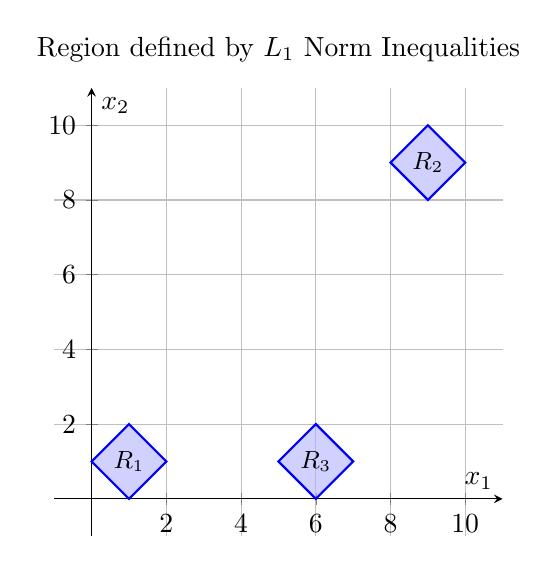
\begin{tikzpicture}
            \begin{axis}[
                % Axis Setup
                axis lines=middle,
                xlabel={$x_1$},
                ylabel={$x_2$},
                xmin=-1, xmax=11,
                ymin=-1, ymax=11,
                grid=major,
                axis equal image, 
                title={Region defined by $L_1$ Norm Inequalities}
            ]

            % --- Region 1 ---
            \filldraw[fill=blue!30, draw=blue, thick, fill opacity=0.6] 
                (axis cs:2,1) -- (axis cs:1,2) -- (axis cs:0,1) -- (axis cs:1,0) -- cycle;
            \node at (axis cs:1,1) {\small $R_1$};

            % --- Region 2 ---
            \filldraw[fill=blue!30, draw=blue, thick, fill opacity=0.6] 
                (axis cs:10,9) -- (axis cs:9,10) -- (axis cs:8,9) -- (axis cs:9,8) -- cycle;
            \node at (axis cs:9,9) {\small $R_2$};

            % --- Region 3 ---
            \filldraw[fill=blue!30, draw=blue, thick, fill opacity=0.6] 
                (axis cs:7,1) -- (axis cs:6,2) -- (axis cs:5,1) -- (axis cs:6,0) -- cycle;
            \node at (axis cs:6,1) {\small $R_3$};

            \end{axis}
        \end{tikzpicture}
        \caption{Visualizing the regions} % Optional caption
    \end{figure}
    \subsection*{Part 2}
    To construct the Big-M formulation, we first linearize the 1-norm constraints. The condition $\|x - C\|_1 \le 1$ can be expressed linearly by introducing auxiliary variables $z_i$ such that $\sum z_i \le 1$ and $|x_i - C_i| \le z_i$.

    Let $b_1, b_2, b_3 \in \{0,1\}$ be binary variables indicating active regions $R_1, R_2, R_3$. We introduce auxiliary variables $z_{k,i} \ge 0$ for each region $k \in \{1,2,3\}$ and dimension $i \in \{1,2,3\}$.

    The Big-M formulation with the smallest valid single $M$ values is derived as follows:
    \begin{itemize}
        \item \textbf{Region 1 ($b_1=1$):} Center $C_1=(1,1,1)$. The maximum distance to a point in $R_2$ is 25, and to $R_3$ is 7. Thus, $M_1 = \max(24, 6) = 24$.
        \item \textbf{Region 2 ($b_2=1$):} Center $C_2=(9,9,9)$. The maximum distance to $R_1$ is 25, and to $R_3$ is 19. Thus, $M_2 = \max(24, 18) = 24$.
        \item \textbf{Region 3 ($b_3=1$):} Center $C_3=(6,1,2)$. The maximum distance to $R_1$ is 7, and to $R_2$ is 19. Thus, $M_3 = \max(6, 18) = 18$.
    \end{itemize}

    The formulation is:

    \[
    \begin{aligned}
        % Region 1 Constraints
        & \text{Region 1:} \\
        & \sum_{i=1}^3 z_{1,i} \leq 1 + 24(1-b_1) \\
        & -z_{1,i} \leq x_i - 1 \leq z_{1,i} \quad \forall i \in \{1,2,3\} \\
        \\
        % Region 2 Constraints
        & \text{Region 2:} \\
        & \sum_{i=1}^3 z_{2,i} \leq 1 + 24(1-b_2) \\
        & -z_{2,i} \leq x_i - 9 \leq z_{2,i} \quad \forall i \in \{1,2,3\} \\
        \\
        % Region 3 Constraints
        & \text{Region 3:} \\
        & \sum_{i=1}^3 z_{3,i} \leq 1 + 18(1-b_3) \\
        & -z_{3,1} \leq x_1 - 6 \leq z_{3,1} \\
        & -z_{3,2} \leq x_2 - 1 \leq z_{3,2} \\
        & -z_{3,3} \leq x_3 - 2 \leq z_{3,3} \\
        \\
        % Global Constraints
        & b_1 + b_2 + b_3 = 1 \\
        & 0 \le x_1, x_2, x_3 \le 10 \\
        & z_{k,i} \ge 0, \quad b_k \in \{0,1\}
    \end{aligned}
    \]

    \subsection*{Part 3: Improved (Lifted) Big-M Formulation}

    To strengthen the continuous relaxation, we apply the lifting procedure to calculate specific Big-M coefficients for each region, rather than using a single global worst-case value.

    Let us define the disjunctive constraints for region $R_k$ as $g_k(x) \le 0$. In the standard Big-M, we used $g_k(x) \le M(1-y_k)$. This is equivalent to $g_k(x) \le M \sum_{j \ne k} y_j$.
    The improved formulation replaces this with:
    \[ g_k(x) \le \sum_{j=1}^3 M_{k,j} y_j \]
    where $M_{k,j}$ represents the amount by which the constraint defining Region $k$ needs to be relaxed to be valid in Region $j$.

    \subsubsection*{1. Calculation of Coefficients}
    We calculate $M_{k,j} = \max_{x \in R_j} (g_k(x))$. Since the regions are defined by $L_1$ distances from centers $C_k$, the value $M_{k,j}$ corresponds to the $L_1$ distance between the center of region $k$ ($C_k$) and region $j$ ($C_j$), as the radius of the target region is 1 and the constraint allows a radius of 1.

    \begin{itemize}
        \item \textbf{Constraints for Region 1 ($C_1=(1,1,1)$):}
        \begin{itemize}
            \item $M_{1,1} = 0$ (Valid in own region).
            \item $M_{1,2} = \|C_1 - C_2\|_1 = 24$.
            \item $M_{1,3} = \|C_1 - C_3\|_1 = 6$.
        \end{itemize}
        \item \textbf{Constraints for Region 2 ($C_2=(9,9,9)$):}
        \begin{itemize}
            \item $M_{2,1} = \|C_2 - C_1\|_1 = 24$.
            \item $M_{2,2} = 0$.
            \item $M_{2,3} = \|C_2 - C_3\|_1 = 18$.
        \end{itemize}
        \item \textbf{Constraints for Region 3 ($C_3=(6,1,2)$):}
        \begin{itemize}
            \item $M_{3,1} = \|C_3 - C_1\|_1 = 6$.
            \item $M_{3,2} = \|C_3 - C_2\|_1 = 18$.
            \item $M_{3,3} = 0$.
        \end{itemize}
    \end{itemize}

    \subsubsection*{2. Resulting Formulation}
    Using the linearized variables $z_{k,i}$ from Part 2, the improved constraints are:

    \[
    \begin{aligned}
        & \text{Constraints defining } R_1: \\
        & \sum_{i=1}^3 z_{1,i} \leq 1 + \mathbf{0}y_1 + \mathbf{24}y_2 + \mathbf{6}y_3 \\
        & -z_{1,i} \leq x_i - 1 \leq z_{1,i} \quad \forall i \\
        \\
        & \text{Constraints defining } R_2: \\
        & \sum_{i=1}^3 z_{2,i} \leq 1 + \mathbf{24}y_1 + \mathbf{0}y_2 + \mathbf{18}y_3 \\
        & -z_{2,i} \leq x_i - 9 \leq z_{2,i} \quad \forall i \\
        \\
        & \text{Constraints defining } R_3: \\
        & \sum_{i=1}^3 z_{3,i} \leq 1 + \mathbf{6}y_1 + \mathbf{18}y_2 + \mathbf{0}y_3 \\
        & -z_{3,i} \leq x_i - C_{3,i} \leq z_{3,i} \quad \forall i
    \end{aligned}
    \]

        \subsubsection*{3. Discussion and Analysis}

        \textbf{Motivation for Strength:} \\
        The improved formulation is stronger because it uses tighter coefficients. In the standard Big-M formulation for Region 1, the term was $24(1-y_1) = 24y_2 + 24y_3$. The improved formulation uses $24y_2 + 6y_3$. Whenever the continuous relaxation assigns a non-zero value to $y_3$ (e.g., $y = (0, 0.5, 0.5)$), the RHS of the improved constraint is smaller ($24(0.5) + 6(0.5) = 15$) than the standard formulation ($24(0.5) + 24(0.5) = 24$), effectively cutting off more infeasible fractional solutions.

        \textbf{Coefficient for the own variable ($M_i$):} \\
        We do not need to compute the coefficient $M_i$ for the binary variable $y_i$ associated with the constraint's own region. It is always **0**. This is because the constraint must be satisfied exactly when $y_i=1$, meaning no relaxation (slack) is allowed.

        \textbf{Equivalence to Conforti Section 7.2:} \\
        \textbf{Yes}, the resulting inequalities are equivalent to the lifting procedure described in Section 7.2 of "Integer Programming" by Conforti et al..
        In that framework, lifting involves starting with an inequality valid for a restriction (e.g., $y_1=1, y_2=0, y_3=0$) and computing the tightest possible coefficients for the variables fixed to 0 ($y_2, y_3$) to make the inequality globally valid. Solving the optimization problem $M_j = \max (a^\top x - b)$ s.t. $x \in R_j$ is exactly the separation problem required to determine these lifting coefficients.
\end{document}